%!TEX program = xelatex

\documentclass[11pt,titlepage]{report}
%!TEX root = main.tex

\usepackage[T1]{fontenc}
\usepackage{lmodern}
\usepackage[svgnames]{xcolor}
\usepackage{fontspec} % XeLaTeX required!
\usepackage{graphicx}
\usepackage{circuitikz}
\usepackage{tikz}
\usepackage{pifont}
\usepackage[some]{background}
\usepackage{xltxtra} 
\usepackage{setspace}
\usepackage[absolute]{textpos}
\usepackage[latin1]{inputenc}
\usepackage[english]{babel}
\usepackage{graphicx}
\usepackage{wrapfig}
\usepackage{fullpage}
\usepackage[margin=1in]{geometry}
\usepackage{float}
\usepackage{url}
\usepackage{multicol}
\usepackage{hyperref}
\usepackage{titlepic}
\usepackage{standalone}
\usepackage{siunitx}
\usepackage{booktabs}
\usepackage{amsmath}
\usepackage{unicode-math}
\usepackage{verbatim}
\usepackage{enumitem}
\usepackage{listings}
\usepackage{multirow}
\usepackage{pgfplots}
\pgfplotsset{compat=1.8}
\usepackage{caption} 
\usepackage[parfill]{parskip}
\usepackage{import}
\usepackage[backend=bibtexu,texencoding=utf8,bibencoding=utf8,style=ieee,sortlocale=en_GB,language=auto]{biblatex}
\usepackage[strict,autostyle]{csquotes}
\usepackage[final]{pdfpages}
\usepackage{subcaption}
\usepackage{ifplatform}
%\captionsetup[table]{skip=10pt}


% Fix for includepdf bug in Mac OS X
\newcommand{\insertpdfpath}[1]{
	\ifwindows
	\newcommand{\insertpdf}[2]{\includepdf[pages=##1]{##2}}
	\else
	\newcommand{\insertpdf}[2]{\includepdf[pages=##1]{#1/##2}}
	\fi
}

%set fonts
\setmainfont[Ligatures=TeX]{Myriad Pro}
\setmathfont{Asana Math}
\setmonofont{Lucida Console}

\usepackage{titlesec, color}
\renewcommand{\familydefault}{\sfdefault} %set font family
\renewcommand{\arraystretch}{1.2} %set table vertical spacing
\setlength\parindent{0pt} %no paragraph indent
\hypersetup{ %setup hyperlinks
    colorlinks,
    citecolor=black,
    filecolor=black,
    linkcolor=black,
    urlcolor=black
}

%redesign chapter headings
\definecolor{gray75}{gray}{0.75}
\newcommand{\chapternumber}{\thechapter}
\newcommand{\hsp}{\hspace{20pt}}
\titleformat{\chapter}[hang]{\Huge\bfseries}{\chapternumber\hsp\textcolor{gray75}{|}\hsp}{0pt}{\Huge\bfseries}

%Redefine appendix headers
\renewcommand{\appendixname}{Appendix}
\renewcommand{\appendixtocname}{Appendices}
\renewcommand{\appendixpagename}{Appendices}

%For code listings
\definecolor{black}{rgb}{0,0,0}
\definecolor{browntags}{rgb}{0.65,0.1,0.1}
\definecolor{bluestrings}{rgb}{0,0,1}
\definecolor{graycomments}{rgb}{0.4,0.4,0.4}
\definecolor{redkeywords}{rgb}{1,0,0}
\definecolor{bluekeywords}{rgb}{0.13,0.13,0.8}
\definecolor{greencomments}{rgb}{0,0.5,0}
\definecolor{redstrings}{rgb}{0.9,0,0}
\definecolor{purpleidentifiers}{rgb}{0.01,0,0.01}


\lstdefinestyle{csharp}{
language=[Sharp]C,
showspaces=false,
showtabs=false,
breaklines=true,
showstringspaces=false,
breakatwhitespace=true,
escapeinside={(*@}{@*)},
columns=fullflexible,
commentstyle=\color{greencomments},
keywordstyle=\color{bluekeywords}\bfseries,
stringstyle=\color{redstrings},
identifierstyle=\color{purpleidentifiers},
basicstyle=\ttfamily\small}

\lstdefinestyle{c}{
language=C,
showspaces=false,
showtabs=false,
breaklines=true,
showstringspaces=false,
breakatwhitespace=true,
escapeinside={(*@}{@*)},
columns=fullflexible,
commentstyle=\color{greencomments},
keywordstyle=\color{bluekeywords}\bfseries,
stringstyle=\color{redstrings},
identifierstyle=\color{purpleidentifiers},
}

\lstdefinestyle{matlab}{
language=Matlab,
showspaces=false,
showtabs=false,
breaklines=true,
showstringspaces=false,
breakatwhitespace=true,
escapeinside={(*@}{@*)},
columns=fullflexible,
commentstyle=\color{greencomments},
keywordstyle=\color{bluekeywords}\bfseries,
stringstyle=\color{redstrings},
identifierstyle=\color{purpleidentifiers}
}

\lstdefinestyle{vhdl}{
language=VHDL,
showspaces=false,
showtabs=false,
breaklines=true,
showstringspaces=false,
breakatwhitespace=true,
escapeinside={(*@}{@*)},
columns=fullflexible,
commentstyle=\color{greencomments},
keywordstyle=\color{bluekeywords}\bfseries,
stringstyle=\color{redstrings},
identifierstyle=\color{purpleidentifiers}
}

\lstdefinestyle{xaml}{
language=XML,
showspaces=false,
showtabs=false,
breaklines=true,
showstringspaces=false,
breakatwhitespace=true,
escapeinside={(*@}{@*)},
columns=fullflexible,
commentstyle=\color{greencomments},
keywordstyle=\color{redkeywords},
stringstyle=\color{bluestrings},
tagstyle=\color{browntags},
morestring=[b]",
  morecomment=[s]{<?}{?>},
  morekeywords={xmlns,version,typex:AsyncRecords,x:Arguments,x:Boolean,x:Byte,x:Char,x:Class,x:ClassAttributes,x:ClassModifier,x:Code,x:ConnectionId,x:Decimal,x:Double,x:FactoryMethod,x:FieldModifier,x:Int16,x:Int32,x:Int64,x:Key,x:Members,x:Name,x:Object,x:Property,x:Shared,x:Single,x:String,x:Subclass,x:SynchronousMode,x:TimeSpan,x:TypeArguments,x:Uid,x:Uri,x:XData,Grid.Column,Grid.ColumnSpan,Click,ClipToBounds,Content,DropDownOpened,FontSize,Foreground,Header,Height,HorizontalAlignment,HorizontalContentAlignment,IsCancel,IsDefault,IsEnabled,IsSelected,Margin,MinHeight,MinWidth,Padding,SnapsToDevicePixels,Target,TextWrapping,Title,VerticalAlignment,VerticalContentAlignment,Width,WindowStartupLocation,Binding,Mode,OneWay,xmlns:x}
}

\lstdefinestyle{matlab}{
language=Matlab,
showspaces=false,
showtabs=false,
breaklines=true,
showstringspaces=false,
breakatwhitespace=true,
escapeinside={(*@}{@*)},
columns=fullflexible,
commentstyle=\color{greencomments},
keywordstyle=\color{bluekeywords}\bfseries,
stringstyle=\color{purpleidentifiers},
identifierstyle=\color{purpleidentifiers}
}

%defaults
\lstset{
basicstyle=\ttfamily\small,
extendedchars=false,
numbers=left,
numberstyle=\ttfamily\tiny,
stepnumber=1,
tabsize=4,
numbersep=5pt
}
\addbibresource{../../library/bibliography.bib}

\begin{document}

\section{Labday 2}
\subsection{Report 8}
For our training sequence, an autocorrelation sequence with an impulse-like characteristic is desirable. This enables us to specifically detect our own sequence, whilst filtering out any interference, like random noise or the signals of any of the other vehicles. 

\begin{figure}[H]
	\centering
	\begin{subfigure}{0.49\textwidth}
		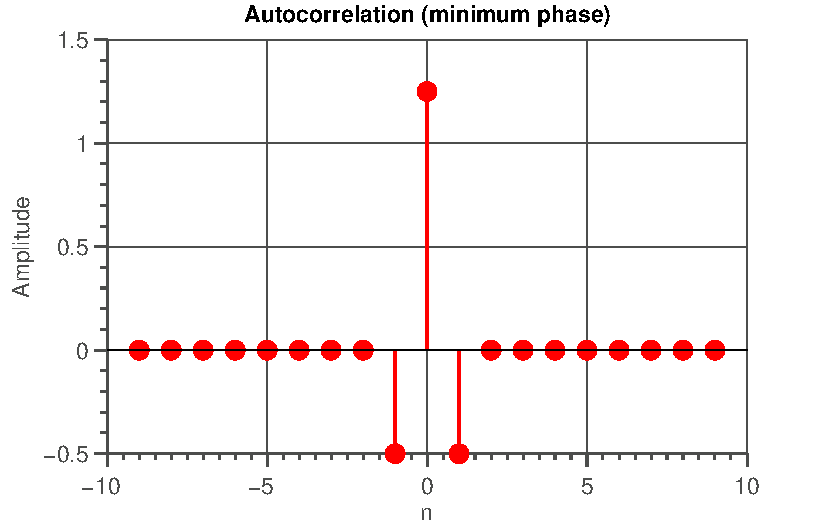
\includegraphics[width=\textwidth]{../../deliverable-7-resources/figures/ass-1/report-8-9-10/report-8/ass-1-report-8-minimum-phase-minimum-phase.pdf}
	\end{subfigure}
	\begin{subfigure}{0.49\textwidth}
		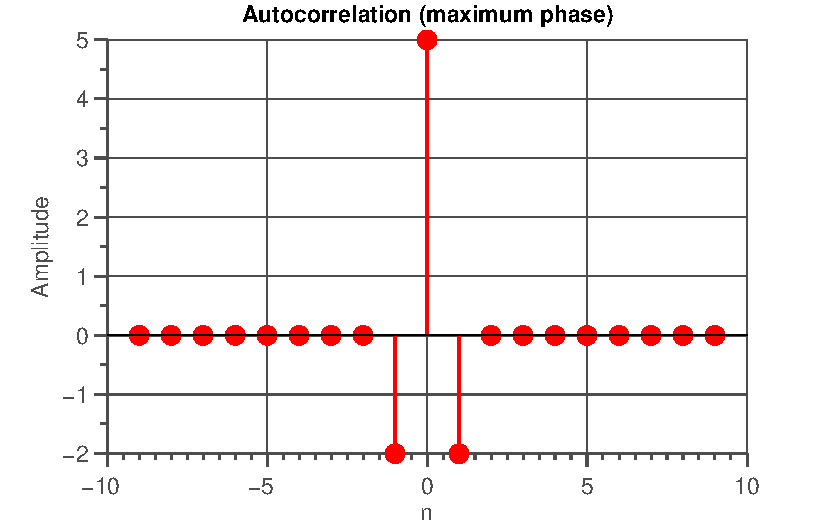
\includegraphics[width=\textwidth]{../../deliverable-7-resources/figures/ass-1/report-8-9-10/report-8/ass-1-report-8-maximum-phase-maximum-phase.pdf}
	\end{subfigure}
	\begin{subfigure}{0.49\textwidth}
		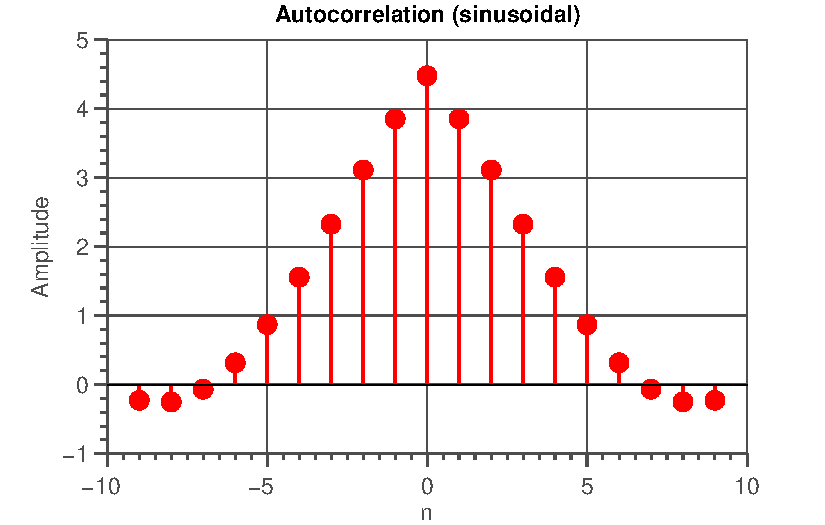
\includegraphics[width=\textwidth]{../../deliverable-7-resources/figures/ass-1/report-8-9-10/report-8/ass-1-report-8-sinusoidal-sinusoidal.pdf}
	\end{subfigure}
	\begin{subfigure}{0.49\textwidth}
		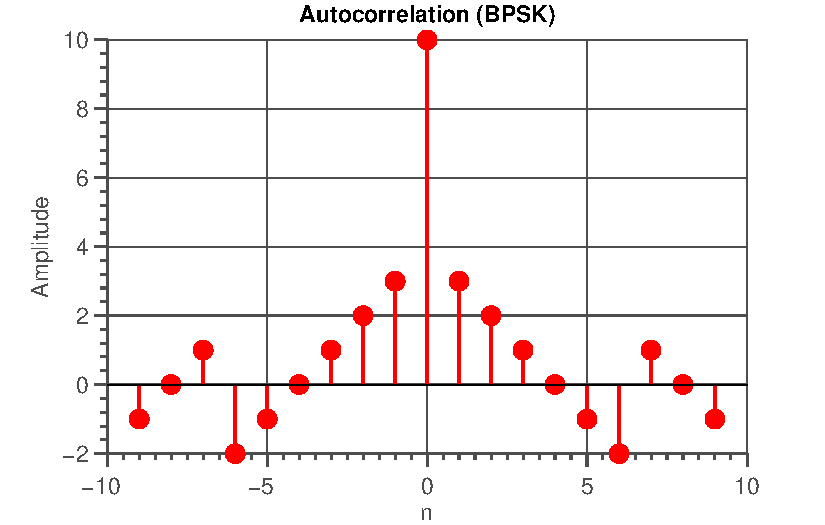
\includegraphics[width=\textwidth]{../../deliverable-7-resources/figures/ass-1/report-8-9-10/report-8/ass-1-report-8-BPSK-BPSK.pdf}
	\end{subfigure}
	\caption{Autocorrelation sequences for each of the tested signals}
	\label{fig:rep8-autocor}
\end{figure}

Figure~\ref{fig:rep8-autocor} shows the autocorrelation sequences of the used signals. We see that both minimum- and maximum-phase sequences exhibit impulse-like behavior, although the maximum-phase sequence's magnitude is about three times as high overall. While this is desirable for the peak at the origin, it also means that the side lobes are larger than the ones of the minimum-phase signal. It is therefore hard to say which signal will perform best, just by looking at this diagram. Looking at the sine and random-BPSK autocorrelation sequences, we observe that they hardly make good candidates for being a training sequence, due to their relatively widespread (non-impulse-like) characteristics.

\subsection{Report 9}

\begin{figure}[H]
	\centering
	\begin{subfigure}{0.49\textwidth}
		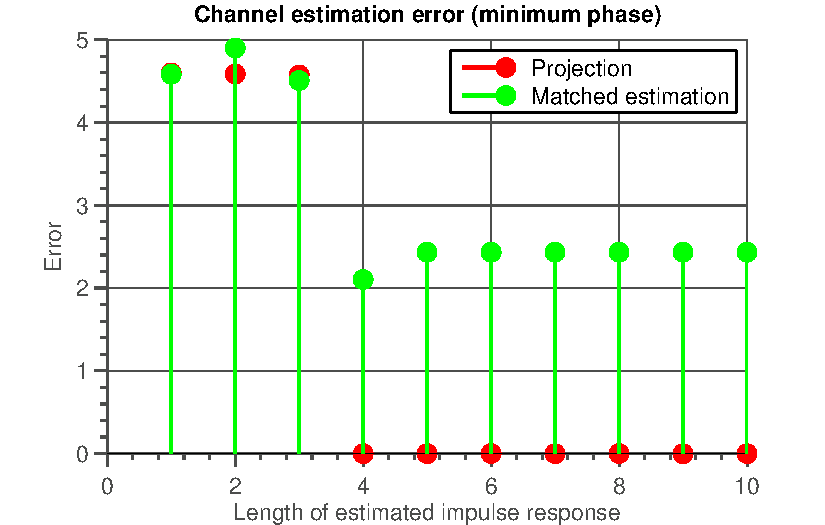
\includegraphics[width=\textwidth]{../../deliverable-7-resources/figures/ass-1/report-8-9-10/report-9-no-noise/ass-1-report-9-minimum-phase.pdf}
	\end{subfigure}
	\begin{subfigure}{0.49\textwidth}
		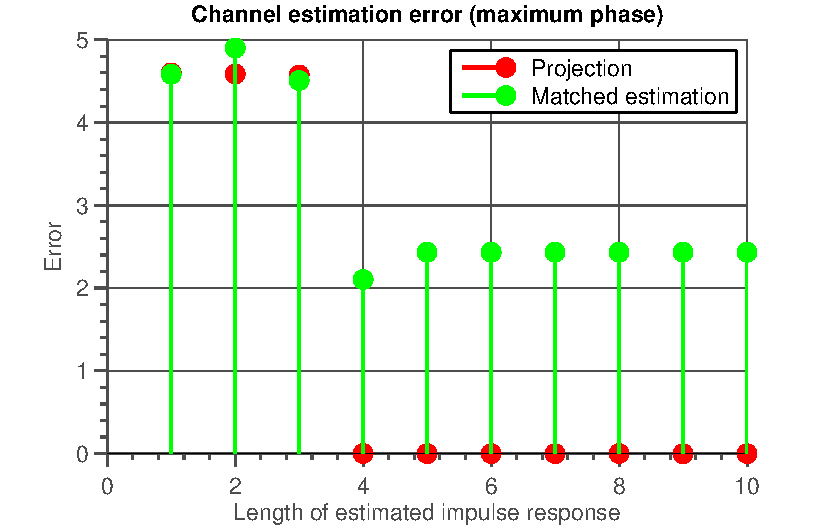
\includegraphics[width=\textwidth]{../../deliverable-7-resources/figures/ass-1/report-8-9-10/report-9-no-noise/ass-1-report-9-maximum-phase.pdf}
	\end{subfigure}
	\begin{subfigure}{0.49\textwidth}
		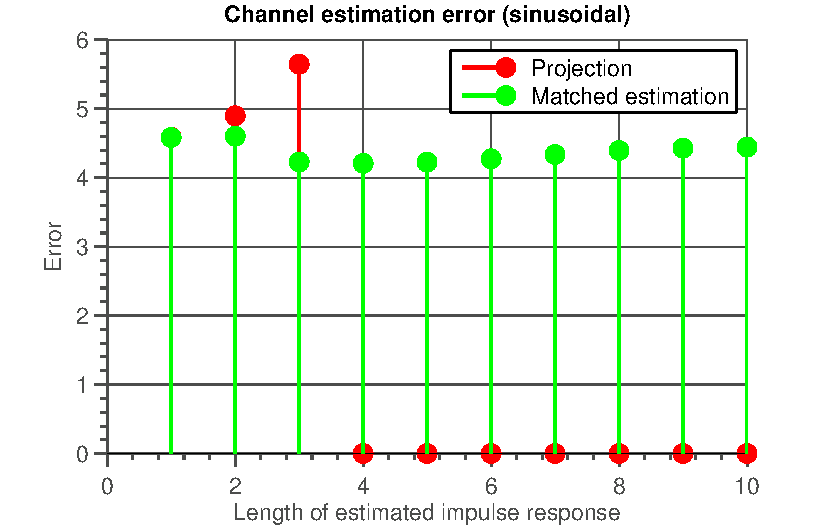
\includegraphics[width=\textwidth]{../../deliverable-7-resources/figures/ass-1/report-8-9-10/report-9-no-noise/ass-1-report-9-sinusoidal.pdf}
	\end{subfigure}
	\begin{subfigure}{0.49\textwidth}
		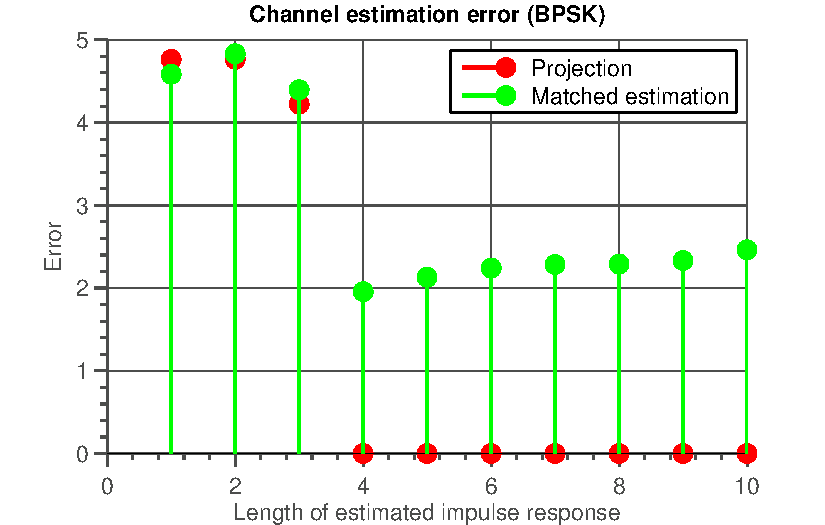
\includegraphics[width=\textwidth]{../../deliverable-7-resources/figures/ass-1/report-8-9-10/report-9-no-noise/ass-1-report-9-BPSK.pdf}
	\end{subfigure}
	\caption{The channel estimation error for increasing $\hat{L}$, without noise}
	\label{fig:rep9-error}
\end{figure}

Figure~\ref{fig:rep9-error} depicts the channel estimation error for each of the four test signals with increasing estimated channel length $\hat{L}$ and without any noise added. We see that for $\hat{L} \ge L = 4$, the inversion/projection estimation method outperforms the matched filter in every case. This is expected behavior since the projection method is supposed to give perfect results in situations without noise and sufficient estimated channel length, where the matched filter sacrifices estimation accuracy for faster performance due to less complex calculations.
However, were we to choose $\hat{L} < L$, we see that it could actually be good to pick the matched-filter approach, since it results in slightly less error in certain situations. Of course, looking at the difference in error between $\hat{L} < L$ and $\hat{L} \ge L = 4$, it would be best to avoid choosing $\hat{L}$ to be too small all together.
Observing the difference between the various signals themselves, we note that the sine and BPSK signals tend to exhibit a slightly smaller error than the minimum- and maximum-phase signals.

\begin{figure}[H]
	\centering
	\begin{subfigure}{0.49\textwidth}
		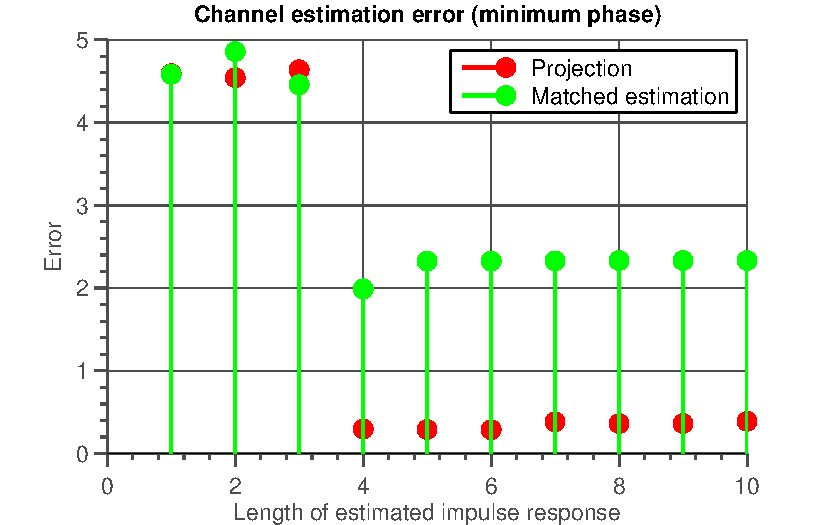
\includegraphics[width=\textwidth]{../../deliverable-7-resources/figures/ass-1/report-8-9-10/report-9-noise-0.1/ass-1-report-9-minimum-phase.pdf}
	\end{subfigure}
	\begin{subfigure}{0.49\textwidth}
		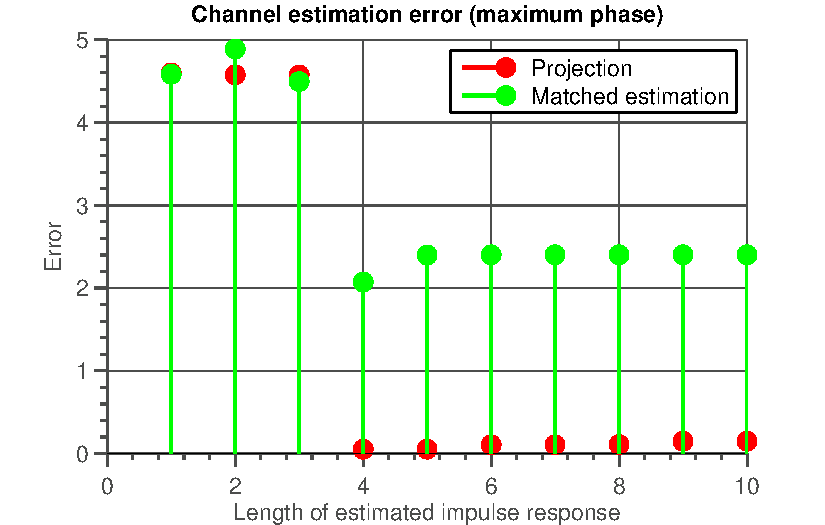
\includegraphics[width=\textwidth]{../../deliverable-7-resources/figures/ass-1/report-8-9-10/report-9-noise-0.1/ass-1-report-9-maximum-phase.pdf}
	\end{subfigure}
	\begin{subfigure}{0.49\textwidth}
		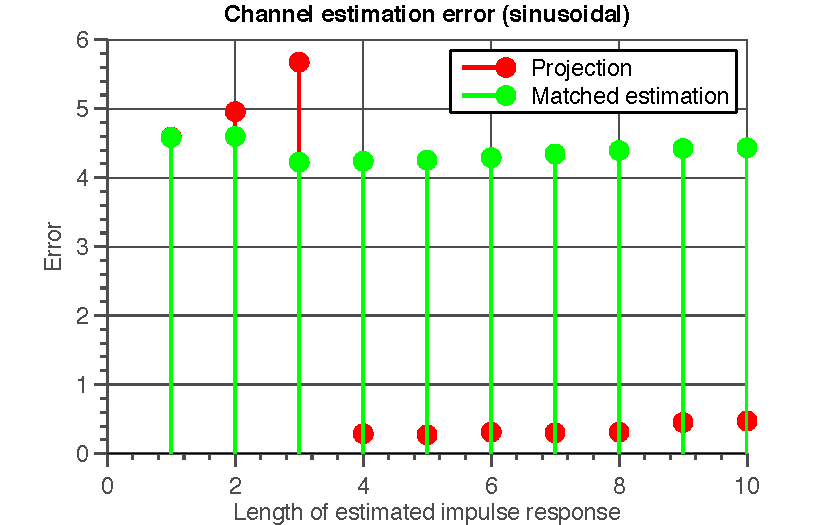
\includegraphics[width=\textwidth]{../../deliverable-7-resources/figures/ass-1/report-8-9-10/report-9-noise-0.1/ass-1-report-9-sinusoidal.pdf}
	\end{subfigure}
	\begin{subfigure}{0.49\textwidth}
		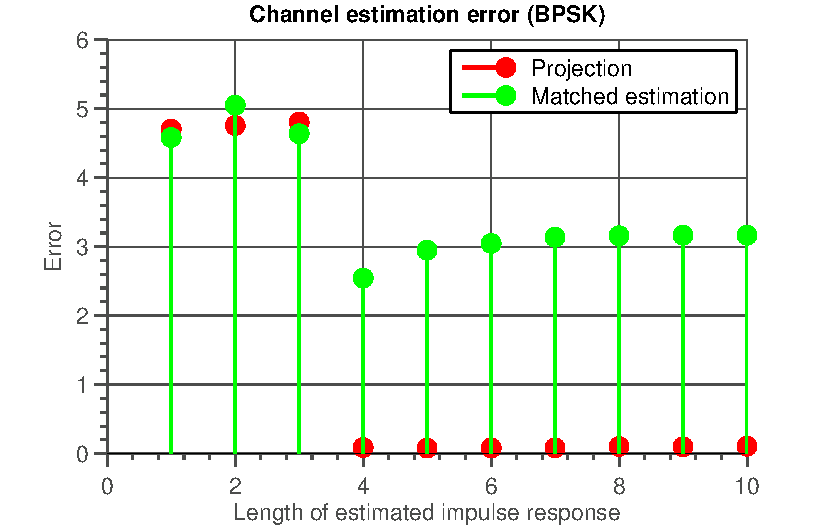
\includegraphics[width=\textwidth]{../../deliverable-7-resources/figures/ass-1/report-8-9-10/report-9-noise-0.1/ass-1-report-9-BPSK.pdf}
	\end{subfigure}
	\caption{The channel estimation error for increasing $\hat{L}$, with noise}
	\label{fig:rep9-error-noise}
\end{figure}

Repeating the previous simulation with added noise with variance $\sigma = 0.1$, as shown in Figure~\ref{fig:rep9-error-noise}, we see nothing spectacular. Both estimation methods now show increased error for all $\hat{L}$, which is to be expected. 

\subsection{Report 10}
The main goal in the design of our training sequence is to be able to perfectly identify it as being ours under every circumstance. This includes noise and other sounds (signals) in the medium. To accomplish this, we want the signal itself to have a high, impulse-like autocorrelation sequence and very low cross-correlation with any arbitrary other signal to avoid interference.
When determining the signal length $N_x$, we take into account that a larger length results in a more unique signal, with better correlation properties, while at the same time it will reduce the maximum tracking speed, since a longer signal takes more time to transmit.
We also noted that it is absolutely crucial to pick a channel length $\hat{L}$ which is at least equal to $L$ itself. Moreover, we would prefer to pick $\hat{L}$ so that $\hat{L} = L$. This way, we may achieve optimal channel estimation, without introducing any calculation overhead due to matrices that are larger than necessary.

\end{document}